\section{Technical Overview}

We now walk the reader through a high-level overview of corrective synchronization with an example. We  describe the conceptual details at a technical level, and then the two main algorithmic steps.

\smartpar{Running Example}
%
As an illustrative example, we refer to the code fragment
below on the
%Figure \ref{Fi:introMotivating},
right,
extracted from the {\sf dyuproject},\footnote{\url{https://code.google.com/archive/p/dyuproject/}} where a shared {\sf Map} object, (pointed-to by) {\sf \_convertors}, is manipulated by method {\sf getConvertor}.\footnote{The code in is a variation of the original code of {\sf dyuproject} where we simplified the syntax for the sake of clarity}
%
%\begin{figure}
%	\begin{lstlisting}[numbers=left]
%public Convertor getConvertor(
%      Class cls,boolean create,boolean add) {
%  Convertor convertor = _convertors.get(cls.getName());
%  if(convertor==null && create) {
%    convertor = new Convertor(cls,add);
%    _convertors.putIfAbsent(cls.getName(), convertor); }
%    return convertor; }
%	\end{lstlisting}
%	\caption{\label{Fi:introMotivating}Method {\sf getConvertor()} from class {\sf StandardConvertorCache} in project {\sf dyuproject}}
%\end{figure}
%
Let us assume that different threads invoking this method
are all attempting to simultaneously obtain the
\begin{wrapfigure}[8]{r}{0.55\textwidth}
%\vspace{-1cm}
  \begin{quote}
	\begin{lstlisting}[numbers=left]
getConvertor(String name, bool create) {
  Convertor conv = _convertors.get(name);
  if(conv==null && create) {
    conv = new Convertor(name);
    _convertors.putIfAbsent(name, conv); }
  return conv; }
	\end{lstlisting}
        \end{quote}
%	\caption{\label{Fi:introMotivating} {\sf getConvertor()} from class {\sf StandardConvertorCache} in {\sf dyuproject}}
\end{wrapfigure}
%
{\sf Convertor} object related to the same key, which is not yet part of the map. Doing so optimistically would lead to multiple rollbacks (even under boosted conflict detection \cite{ppopp08}, since the operations due to different threads do not commute), and thus poor performance. Pessimistic mutual exclusion, on the other hand, would block all but one thread until the operation completes, which is far from optimal if {\sf new Convertor()} is an expensive operation.


%%%%%%%%%%%%%%%%

\newcommand\hrel{\sim}
\smartpar{Conceptual Approach}
%
By \emph{corrective synchronization} we mean the ability to transform a concurrent run that, in its present condition, may not be serializable into a run that is serializable. Stated formally, corrective synchronization is a relationship $h \hrel h'$ between histories, such that (i) $h$ and $h'$ share the same initial state, and (ii) $h$ and $h'$ share the same log of committed operations (i.e., they agree on the operations on the shared-state). One can think of $h'$ as an alternate parallel reality to $h$.

The first condition ensures that corrective synchronization yields a feasible outcome. The second is the requirement not to roll back updates to the shared state. These two conditions distinguish corrective synchronization from existing solutions: Unlike pessimistic approaches, bad behaviors may occur under corrective synchronization. That is, they are not avoided, but handled as they manifest. Unlike optimistic solutions, the core handling mechanism is not to retry the transaction (or parts thereof), which implies rolling back (either committed or uncommitted) updates to the shared log, but rather to ``warp'' to another state.
%
To illustrate our approach, consider the following  history: % in Figure \ref{Fi:motivatingInterleaving}.
	\begin{center}
		\begin{tabular}{r@{}lrcl@{}l}
			[ & & $T_1$: ${\sf get()}/{\sf null}$ & $\rightarrow$ & $T_2$: ${\sf get()}/{\sf null}$  & \\
			& $\hookrightarrow$ & $T_1$: ${\sf if(\ldots)}$ & $\rightarrow$  & $T_2$: ${\sf if(\ldots)}$ & \\ 
			& $\hookrightarrow$ & $T_1$: ${\sf new\ \ldots}/o_1$ & $\rightarrow$ & $T_2$: ${\sf new\ \ldots}/o_2$ & \\ 
			& $\hookrightarrow$ & $T_1$: ${\sf putIfAbsent()}/{\sf null}$ & $\rightarrow$ & $T_2$: ${\sf putIfAbsent()}/o_1$  & \\ 
			& $\hookrightarrow$ & $T_1$: ${\sf return}\ o_1$ & $\rightarrow$ & $T_2$: ${\sf return}\ o_2$ & ]
		\end{tabular}
	\end{center}
Each step in this history is labeled with the transaction identifier ($T_1$ or $T_2$) and the code that the transaction is executing.
This history is clearly not serializable. In any serializable history, $T_1$ and $T_2$ would return the same {\sf Convertor} instance. However, we can warp to such a serializabile history by applying a correction.
%
Correcting this execution involves the application of two actions to the exit state of $T_2$. First, we point the local variable ${\sf conv}$ to $o_1$, rather than $o_2$. Second, we fix the mapping under ${\sf \_convertors}$ for key {\sf name} in the same way.
%
Note that the corrective actions above are of a general form, which is not limited to two threads. For any number of threads, the corrected state would have one privileged thread deciding the return value (i.e., the value of {\sf conv}) for all threads, which would also be the value linked by the key under {\sf \_convertors}.

How does this corrective approach compare to handling of the situation by pessimistic or optimistic approaches?
%
We illustrate the difference between corrective synchronization and classic optimistic and pessimistic synchronization in Figure \ref{Fi:motivatingOverview}. We visually represent concurrent execution of two instances of the \textsf{getConvertor} code using pessimistic locks, optimistic TM and corrective synchronization (proceeding horizontally left-to-right). Pessimism serializes execution, and so there is no performance gain whatsoever. As for optimistic and corrective synchronization, we consider the interleaving scenario specified above. % from Figure \ref{Fi:motivatingInterleaving}. 
%
\begin{figure*}[t]
	\begin{center}
	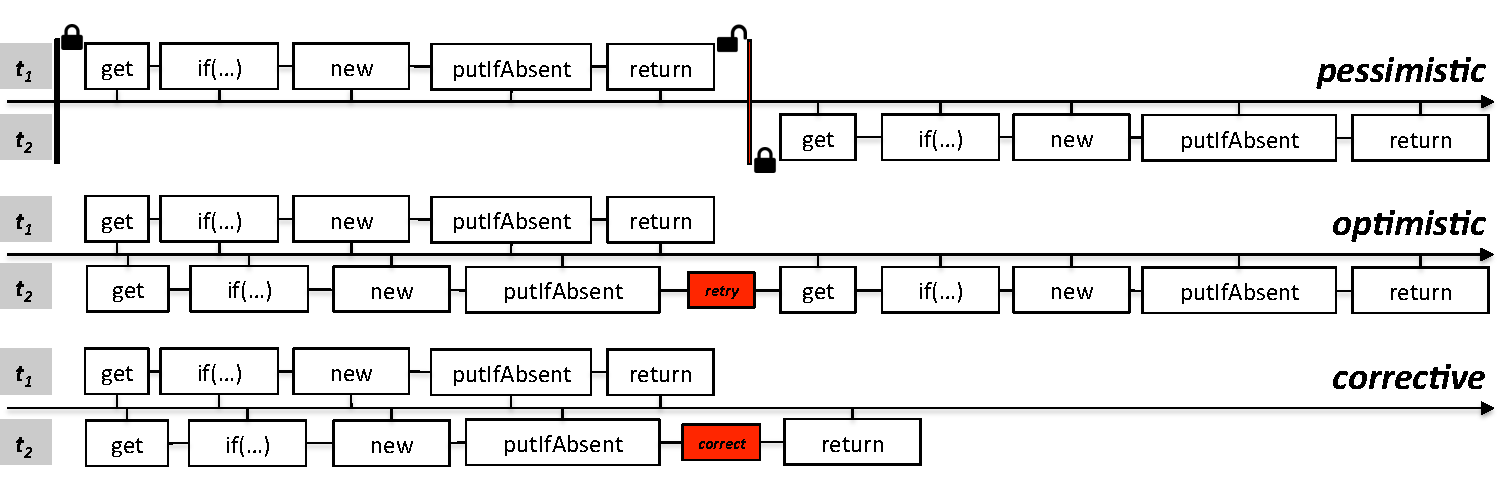
\includegraphics[width=\textwidth]{OverviewSlide.pdf}
	\end{center}
	\vspace{-0.6cm}\caption{\label{Fi:motivatingOverview}Interleaved execution of two instances of \textsf{getConvertors} using pessimistic, optimistic, and corrective synchronization.}
        \vspace{-0.4cm}
\end{figure*}
%
Both optimistic and corrective synchronization, allowing the problematic chain of interleavings, reach a nonserializable state. Optimism resolves this by retrying the entire transaction executed by, say, thread $t_2$. This yields serial execution, similar to the pessimistic run, where $t_2$ runs after $t_1$. Corrective synchronization, instead, ``fixes'' the final state, allowing $t_2$ to complete without rerunning any or all of its code.
%
Our experiments suggest the corrective actions are --- relatively speaking --- inexpensive, especially compared to the alternatives of either blocking or aborting/restarting all threads but one.


We refer to corrective synchronization as \emph{sound} if $h'$ is the prefix of a serializable execution of the system. We refer to corrective synchronization as \emph{complete} if for any $h$, all the $h'$s that satisfy the conditions above are in the relation $\hrel$. In the rest of this paper, we describe our method of computing a sound yet incomplete set of corrective targets via static analysis of the concurrent library.
%
A solution that is not complete faces the possibility of stuck runs: Given a (potentially) nonserializable execution prefix, the system does not have a corresponding serializable prefix to transition to. In this paper, we do not present a solution to the completeness problem, which we leave as future work. In the meantime, there are two simple strategies to tackle this problem: (i) \emph{manual specification}, whereby the user completes the set of corrective targets to ensure that there are no stuck runs (in our implementation, the targets are computed offline via static analysis, letting the user complete the specification ahead of deployment); and (ii) \emph{complementary techniques}, such as optimism, which the system can default to in the absence of a corrective target.
%\begin{compactitem}
%	\item Manual specification: The user completes the set of corrective targets computed automatically, such that there are no stuck runs. In our implementation of corrective synchronization, the corrective targets are computed offline via static analysis, which lets the user complete the specification prior to the deployment runs.
%	\item Complementary techniques: In the absence of a corrective target, the system can default to another synchronization technique such as STM. This provides a general means to avoid stuck states without causing any overhead w.r.t. standard techniques.
%\end{compactitem}


\smartpar{Computing Corrective Targets}
%
A simpler and more abstract specification to work with, compared to complete execution prefixes, is triplets $(s,s',s'')$ of states, such that there exist prefixes $h$ and $h'$ as above with respective initial and current states $(s,s')$ and $(s,s'')$, respectively. This form of specification is advantageous, because the corresponding runtime instrumentation is minimal compared to tracking traces. At the same time, however, initial and current states are a strict abstraction of complete traces, and so they do not 
point back to prefixes $h$ and $h'$.

Mapping back from pairs of states to prefixes requires an oracle. In our work we compute the oracle as a relational abstract interpretation solution over the program that is sound yet incomplete. Specifically, an underapproximation of the serializable intermediate (or final) states is computed as the fixpoint solution over an interprocedural control-flow graph (CFG) of the form: 
	$t_1 \rightarrow t^\star_{2 \ldots n} \rightarrow t_{n+1} \rightarrow t'_1 \rightarrow t'^\star_{2 \ldots n} \rightarrow t'_{n+1} \rightarrow \ldots$,
where $t$, $t'$, etc denote different transaction types (i.e., transactions executing different code), and $n$ is unbounded, simulating a nondeterministic loop. This representation simulates an unbounded number of instances of transactions that are executed sequentially.

We go into detail about this representation in Section \ref{sec:transactionsystemwarping}, but here note that (i) this representation reflects the effects of serial execution of the transactions, and so the corrective targets are guaranteed to be sound; (ii) the nondeterministic loop captures an unbounded number of transactions; and (iii) the first and last transactions of a given type are purposely disambiguated to boost the precision of static analysis over the simulated execution.
%
As an illustration of the third point, in our running example the first transaction $t_1$ is modeled precisely in inserting the key/value pair into the {\sf Map} object. Analogously, the last transaction $t_{n+1}$ can be confirmed not to update the key/value mapping.

\smartpar{Runtime Synchronization} 
%
The runtime system has two main responsibilities. First, it must track whether an execution has reached a (potentially) bad state. Second, if such a state arises, then the runtime system must map the current state onto a state that shares the same initial state and is known, by the oracle, to have a serializable continuation. 
%
We address the first challenge via a coarse conflict-detection algorithm that tracks API-level read/write behaviors (at the level of {\sf Map} operations). If read/write or write/write conflicts arise, then corrective synchronization is triggered in response. 

\OmerAdded{The second challenge, of deciding the target ``good'' state for a given ``bad'' state, is tackled via a pruning algorithm. During execution, the system maintains (as shadow state) a set of good symbolic final states. As individual transactions complete, incompatible final states (i.e., states that cannot be reached via any of the computed corrective actions) are pruned out. The remaining states are all guaranteed to be admissible targets. The decision which state to transition to is based on a heuristic measure of the cost of the corrective action (which simply counts the number of basic operations needed).}

We expand on the above challenges in Section \ref{sec:transactionsystemwarping}, and provide encouraging experimental results on a simple prototype in Section~\ref{Se:experiments}. Prior to that, in Section \ref{se:instance}, we provide a formal statement of corrective synchronization.


\OmerAdded{
\subsection{Discussion}
As outlined above, the concrete instance that we have developed of corrective synchronization is specific to loop parallelization (in that transactions begin at the same time) and map clients. This particular setup is already applicable to many real-world codes \cite{oopsla/ShachamBASVY11,issta/ShachamYGABSV14}. Still, we emphasize that there are various natural extensions that widen this scope significantly and we intend to explore in the future.
}

%\OmerAdded{
%	First, there is no need, in general, to focus on maps. Concrete-level transactional memory ranges over variable and field accesses, enabling computation of corrective targets in terms of nonconflicting accesses to shared fields. For this any sound abstraction of runtime objects (e.g. as allocation sites) would suffice.
%}

\OmerAdded{A first extension is to consider additional ADTs, beyond map, such as set and counter \cite{ppopp08}. Assuming encapsulation \cite{TYFS:OOPSLA11}, it becomes possible to compose handling of different ADTs both with each other and with concrete-level corrective synchronization.}

\OmerAdded{The assumption regarding starting times can also be relaxed, albeit at the cost of more expensive offline analysis. While no change is needed to the core analysis algorithm, there are more cases that should be accounted for, namely some (if not all) of the possibilities for transaction $t$ to start when concurrent transaction $t’$ is at a control location in its CFG other than the entry location. In our experimental results, the core analysis algorithm took less than a second to converge. Therefore, we believe that it would be able to explore thousands of combinations within a single hour.}
	
